\section{VL vom 09. November 2010}

\subsection{Beweis Resolutionslemma}

\begin{itemize}
  \item $V \models  M \cup \set{C} \Rightarrow V \models  M$ trivial.
  \item Es gelte $V\models M$. Ferner sei $C=(C_1\backslash \set{\ell}) \cup
  (C_2\backslash \set{\overline{\ell}})$ mit $C_1,C_2 \in M$. Unterscheide zwei
  Fälle:
  \begin{itemize}
    \item $V(\ell) = 1$. Wegen $V\models C_2$ dann auch $V\models C_2\backslash \set{\overline{\ell}}$.
    \item $V(\ell) = 0$. Wegen $V\models C_1$ dann auch $V\models C_1\backslash \set{\overline{\ell}}$.
  \end{itemize}
  In beiden Fällen also $V\models C$.\qed
\end{itemize}

\subsubsection{Beispiel-Resolution}

\begin{align}
  M(\varphi) &= \set{\set{x_1}, \set{\NOT x_1, x_2}, \set{\NOT x_2, x_3}, \set{\NOT x_3}} = M \\
  \Res^0(M)   &= M \\
  \Res^1(M)   &= \Res^0(M) \cup \set{\set{x_2}, \set{\NOT x_1, x_3}, \set{\NOT x_2}} \\
  \Res^2(M)   &= \Res^1(M) \cup \set{\set{x_3}, \set{\NOT x_1}, \square} \\
  \Res^3(M)   &= \Res^2(M) = \Res^*(M)
\end{align}

\subsection{Beweis Resolutionssatz}

\begin{itemize}
  \item[$\Leftarrow$] \textbf{Korrektheit}\par
  Da $\square \in \Res^*(M)$, ist $\Res^*(M)$ unerfüllbar. Es genügt also zu zeigen, dass $\Res^*(M)\EQUIV M$.
  Mittels Resolutionslemma und per Induktion über $i$ zeigt man leicht, dass $M\EQUIV \Res^i(M) \forall i \geq 0$.
  Da sich über den endlich vielen Literalen in $M$ nur endlich viele Klauseln bilden lassen, ist $\Res^*(M)$ endlich, also $\Res^*(M) = \Res^i(M)$ für ein $i\geq 0$, damit $M\EQUIV \Res^*(M)$.
  
  \item[$\Rightarrow$] \textbf{Vollständigkeit}\par
  Wir zeigen
  \[
    M\ \text{unerfüllbar} \IMPL \square \in \Res^*(M)
  \]
  per Induktion über $|\Var(M)|$.
  \begin{description}
    \item[IA] $\Var(M) \not= \emptyset$. Dann $M=\emptyset$ oder $M=\set{\square}$.
    Da $\emptyset$ erfüllbar, muss $M=\set{\square}$ sein, also $\square\in M \subseteq \Res^*(M)$.
    
    \item[IS] Wähle $x\in \Var(M)$, konstruiere zwei Klauselmengen:
    \begin{align}
      K^+ &:= \set{C \backslash \set{\NOT x} | x \not\in C \in M} \\
      K^- &:= \set{C \backslash \set{x} | \NOT x \not\in C \in M} 
    \end{align}
    Intuitiv entspricht $K^+$ dem Fall $V(x) = 1$: alle Klauseln $C$ mit $x \in C$
    sind erfüllt und wurden gestrichen, aus den verbliebenen Klauseln kann
    $\NOT x$ gestrichen werden (wenn vorhanden), denn $\NOT x$ kann die Klausel
    nicht wahr machen.
    
    Wir zeigen:
    \begin{enumerate}
      \item $K^+$ und $K^-$ sind unerfüllbar
      \item $\square \in \Res^*(M)$ oder $\set{\NOT x} \in \Res^*(M)$
      \item $\square \in \Res^*(M)$ oder $\set{x} \in \Res^*(M)$
    \end{enumerate}
    
    \item[(1)] Angenommen, $K^+$ ist erfüllbar und $V\models K^+$.
    Erweitere $V$ durch $V(x)=1$. Man prüft leicht, dass $V\models M$. $\lightning$
    
    Unerfüllbarkeit $K^-$ analog.
    
    \item[(2)] Weil $K^+$ unerfüllbar liefert IV $\square\in\Res^*(K^+)$.
    Also gibt es Klauseln $C_1,\dots,C_m$, so dass $C_m=\square$ und für $1\leq i\leq m$ gilt
    \begin{enumerate}
      \item $C_i \in K^+$ oder
      \item $C_i$ ist Resolvente von $C_j,C_k$ für je gewisse $j,k < i$.
    \end{enumerate}

    \textbf{Fall 1:} alle Klauseln $C_i$ der Form (a) sind auch in $M$ (in keiner der
    \enquote{Originalklauseln} kam $\NOT x$ vor). Dann prüft man leicht, dass
    $C_1,\dots,C_m \in\Res^*(M)$, also $\square\in\Res^*(M)$.
    
    \textbf{Fall 2:} Für mind. ein $C_i$ der Form (a) ist $C_i\cup\set{\NOT x}\in M$.
    Wir erhalten duch Wiedereinfügen von $\NOT x$ eine Folge von Klauseln
    $C'_1,\dots,C'_m \in \Res^*(M)$, die beweist, dass $\set{\NOT x}\in\Res^*(M)$.
    
    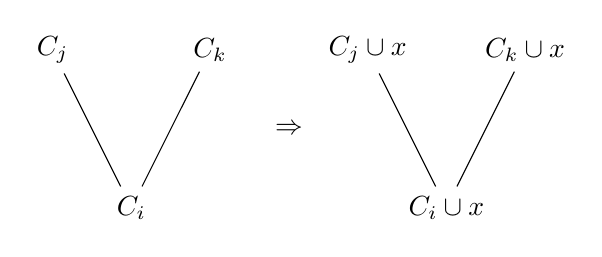
\begin{tikzpicture}
      \node (j) at (-1,1) {$C_j$};
      \node (k) at (1,1) {$C_k$};
      \node (i) at (0,-1) {$C_i$};
      \draw (j)--(i) (k)--(i);
      
      \node at (2,0) {$\Rightarrow$};
      \node (j) at (3,1) {$C_j\cup\set{\NOT x}$};
      \node (k) at (5,1) {$C_k\cup\set{\NOT x}$};
      \node (i) at (4,-1) {$C_i\cup\set{\NOT x}$};
      \draw (j)--(i) (k)--(i);
    \end{tikzpicture}
    \begin{verbatim}
      C_j     C_k       C_j\cup\set{\NOT x}   C_k\cup\set{\NOT x}
         \   /      =>                \          /
          C_i                      C_i\cup\set{\NOT x}
    \end{verbatim}
    \item[(3)] Analog zu (2) unter Verwendung von $K^-$.
  \end{description}
  Aus (2) und (3) folgt, dass $\square\in\Res^*(M)$ oder $\set{x},\set{\NOT x}\in\Res^*(M)$. Mit
  \begin{verbatim}
    \set{\NOT x}     \set{x}
             \         /
               \square
  \end{verbatim}
  dass auch $\square\in\Res^*(M)$.\qed
\end{itemize}
